\startchapter{Analysis Preparation}
\label{chapter:ana_prep}

\section{Signal Model}
This work concerns a search for dark matter produced in association with a dark Higgs boson as described in Section \ref{subsection:dh_model}.  The dark Higgs boson then decays to standard model particles with the same branching ratios as a standard model Higgs boson of variable mass, shown in Figure ~. At low $s$ mass this is dominated by a decay to a pair of $b$ quarks, which has been explored by reinterpreting the ATLAS search for dark matter produced in association with a standard model Higgs boson decaying to $b\bar{b}$. [cite,cite] At $s$ masses above 160 $GeV$, however, the decay to a pair of W bosons, shown in Figure ~ becomes kinematically available on-shell. Even slightly below this threshold, $s$ decays to $WW$ are the dominant process. The pair of W bosons decay rapidly, and are not detected as final state particles by the ATLAS detector. Instead, they each decay either to hadronic ($q\bar{q}$) or leptonic ($l\nu$) final states. A search in the fully hadronic channel, with both $W$ decaying to $q\bar{q}$ is complete, and this work focuses on the semileptonic decay channel with one $ W \rightarrow q\bar{q} $ and one $ W \rightarrow l\nu $. When both analyses are complete, the results will be statistically combined.

\begin{figure}[H]
    \centering
    \feynmandiagram [horizontal=a to b] {
    i1[particle=\(q\)] -- [fermion] a -- [fermion] i2[particle=\(q\)],
    a -- [boson, edge label=\(Z'\)] b,
    b -- [boson, edge label=\(Z'\)] c,
    b -- [scalar, edge label=\(s\)] d,
    f1[particle=\(\chi\)] -- [fermion] c -- [fermion] f2[particle=\(\chi\)],
    f3[particle=\(W\)] -- [boson] d -- [boson] f4[particle=\(W\)],
    f2 -- [opacity=0.0] f3
    };
    \caption{DH Decay}
    \label{fig:dh_feynman}
\end{figure}

In the ATLAS detector this signal signature will be characterized by a single lepton in the final state from the $ W \rightarrow l\nu $ decay, along with a pair of jets from the $ W \rightarrow q\bar{q} $ decay and a strong missing transverse energy signature from the dark matter particles and neutrino.

\section{Monte Carlo Production}
\label{section:mc_prod}
Monte Carlo (MC) simulated samples of both BSM (signal) and SM (background) events were used in this analysis. In this way, potentially signal-rich regions can be prepared and studied separately from real data and then later compared to see whether simulated data and true data agree. The following section will detail the signal and background MC samples used.

\subsection{Signal}
\label{subsection:mc_signal}
Signal samples are produced using the model and parameter choices outlined in Section \ref{subsection:dh_model}. They were produced by calculating the hard process cross-section at leading order (LO) using \mgamc 2.7.2 interfaced with \pythia 8.230 for parton shower modelling. The CKKW-L https://arxiv.org/pdf/1109.4829.pdf procedure with a matching scale of $min(m_s, 40~GeV)$ was used to prevent overlap between the cross-section matrix element and parton shower. Two separate signal grids were produce, with the second covering an expanded parameter space. In the first, \mgamc was used with the NNPDF23 LO PDF set with $\alpha_s = 0.13$, while in the second \mgamc was both used with the NNPDF23 LO PDF set with $\alpha_s = 0.13$ and LO QED. The signals studied span a parameter space in \ms and \mZp with samples produced at the mass points shown in Figure ~. After production, it was found that the second set of samples did not use the ATLAS recommended PDF Set, which is in fact NNPDF23 NLO PDF set with $\alpha_s = 0.118$. When used, the weights of events in these samples are therefore scaled to match the cross-sections of the recommended PDF set.

\begin{figure}[H]
    \centering
    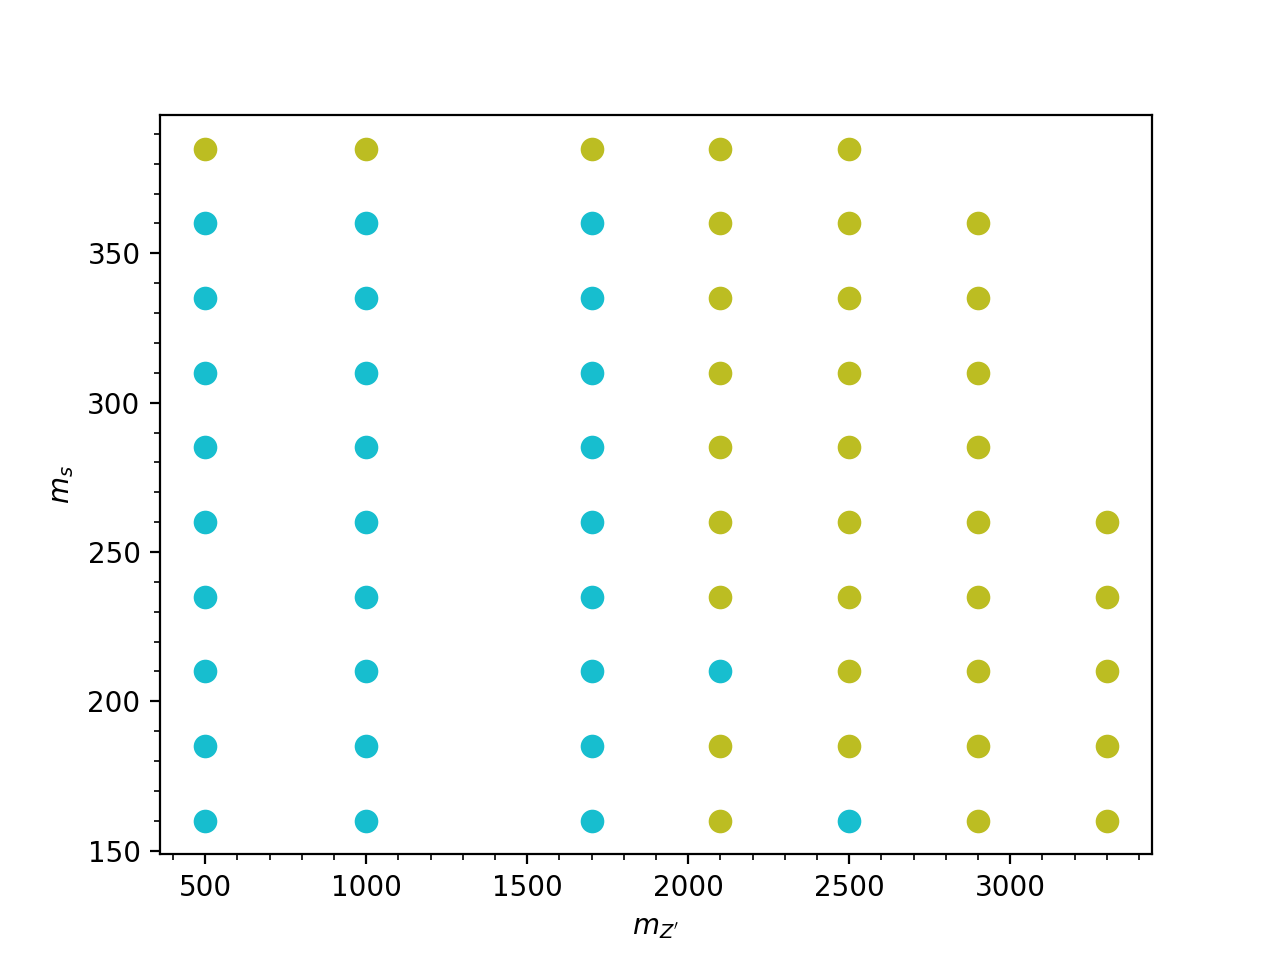
\includegraphics[width=0.8\textwidth]{Figures/3/SignalGrid.png}
    \caption{Signal point locations in \ms vs. \mZp parameter space.}
    \label{fig:signal_grid}
\end{figure}

\subsection{Background}
\label{subsection:mc_bkg}
The dominant SM backgrounds for this analysis are:
\begin{itemize}
    \item \wjets events a single W boson and 1 or more jets,
    \item \ttbar events with a top and anti-top pair,
    \item and \textit{Diboson} events with a pair of vector bosons
\end{itemize}
Additionally, \zjets and single-top quark (stop) events make non-negligible background contributions. All background contributions are estimated using MC simulated data, and the \wjets and \ttbar backgrounds are further constrained using data-driven control regions.

\subsubsection{\vjets and diboson}
Like signal, two distinct sets of \wjets and \zjets (\vjets) background samples were used. The samples are similar in that \wjets and \zjets (\vjets) are simulated with the \sherpa v2.2 MC generator with up to two additional parton emissions at NLO or four additional parton emissions at LO accuracy. Merging of parton showers with matrix elements is acheived using CKKW matching with the MEPS@NLO prescription extending this to NLO. *https://cds.cern.ch/record/2261937/files/ATL-PHYS-PUB-2017-006.pdf* Sect 2.1. The NNPDF30 NNLO https://arxiv.org/pdf/1410.8849.pdf set is used.
The difference is that first samples were produced using \sherpa v2.2.1, and the second with \sherpa v2.2.10. As well, additional \wjets samples are added to the second set with $m_W > 120 GeV$. This greatly enhances the statistics in this small section of phase space that is important to this analysis. Overlap removal in $m_W$ is performed between these mass-enhanced samples and the other \wjets samples. https://cds.cern.ch/record/2753199/files/ATL-COM-PHYS-2021-063.pdf?
Diboson samples are similarly generated with only a single set using either \sherpa v2.2.1 or 2.2.2 depending on the process, and CKKW matching again used to merge parton shower and matrix element simulation.

\subsubsection{\ttbar and single-top}
MC samples for the \ttbar and single-top standard model background process were modelled using the \powhegbox v2 generator, which gives martix elements at NLO in the strong coupling constant $\alpha_s$. This uses the NNPDF3.0NO PDF set. Like for signal samples, events were interfaced with \pythia 8.230 for parton shower modelling using the NNPDF23LO PDF set.

\section{Object Definition}
Once events have been simulated or produced in the ATLAS detector, the information contained in them must be reconstructed into objects which can be analyzed. These objects represent particles or groups of particles and are used to fully or partially reconstruct events and search for signal signatures. The following section will detail the definition of objects used in this analysis.

\subsection{Muons}
From the ATLAS detector, muons are reconstructed from measurements in the Inner Detector and the Muon Spectrometer. For this analysis, two different definitions of muons are used. ``\textit{Baseline}" muons use a slighlty less selective reconstruction than ``\textit{signal}" muons, which are designed for high purity. \textit{Baseline} muons are selected using the \textit{Loose} identification criteria as defined in https://arxiv.org/pdf/1603.05598.pdf, which is designed to maximize efficiency. \textit{Signal} muons, meanwhile, use the \textit{Medium} identification criteria, and must also be isolated according to the \textit{Tight} track-based working point with variable radius dependent on \pT. Additionally, all muons are rejected if they are considered ``badly reconstructed" or ``cosmic", and recommended track-to-vertex association cuts are applied. Table \ref{tab:muon_criteria} summarizes the muon selection criteria.

\begin{table}[htbp]
\centering
\caption{Muon object definition criteria}
\label{tab:muon_criteria}
\begin{tabular}{l l l}
\toprule
\textbf{Criterion} & \textbf{Baseline Muon} & \textbf{Signal Muon} \\
\midrule
Identification & \verb|Loose| & \verb|Medium| \\
Isolation & - & \verb|TightTrackOnly_VarRad| \\
\midrule
Pseudorapidity & \(\abs{\eta} < 2.7\) & \(\abs{\eta} < 2.5\) \\
\pT & \(\pT > \unit[7]{\GeV} \) & \(\pT> \unit[7]{\GeV} \) \\
\midrule
Veto & Cosmic or Bad & Cosmic or Bad \\
\midrule
\multirow{2}{*}{Track-to-vertex association} & \(\abs{d_0 / \sigma_{d_0}}  < 3 \) & \( \abs{d_0 / \sigma_{d_0}}  < 3 \) \\
	& \( \abs{\Delta z_0^\textrm{BL} \sin \theta} < \unit[0.5]{mm} \) & \( \abs{\Delta z_0^\textrm{BL} \sin \theta} < \unit[0.5]{mm} \) \\
\bottomrule
\end{tabular}
\end{table}

\subsection{Electrons}
Electrons are reconstructed by associating energy deposits in the EM calorimeter with tracks in the inner detector. Like for muons, two different definitions are used, with ``\textit{baseline}" electrons requiring slighlty less selective criteria than ``\textit{signal}" electrons. \textit{Baseline} and \textit{signal} electrons are selecteded using a likelihood-based identification described in https://arxiv.org/pdf/1902.04655.pdf. \textit{Signal} electrons require the medium identification criteria, while \textit{baseline} electrons requre the loose criteria as well as a hit in the innermost layer of the pixel detector. Additionally, \textit{baseline} and \textit{signal} electrons must both satisfy the fixed-cut \textit{Loose} isolation requirement. Like for muons, ATLAS recommended track-to-vertex association cuts are applied. Table \ref{tab:electron_criteria} summarizes the electron selection criteria.

\begin{table}[htbp]
\centering
\caption{Electron object definition criteria}
\label{tab:electron_criteria}
\begin{tabular}{l l l}
\toprule
\textbf{Criterion} & \textbf{Baseline Electron} & \textbf{Signal Electron} \\
\midrule
Identification & \verb|LooseAndBLayerLLH| & \verb|MediumLLH| \\
Isolation & \verb|FCLoose| & \verb|FCLoose| \\
\midrule
Pseudorapidity & \(\abs{\eta} < 2.47\) & \(\abs{\eta} < 2.47\) \\
\pT & \(\pT > \unit[7]{\GeV} \) & \(\pT> \unit[7]{\GeV} \) \\
\midrule
\multirow{2}{*}{Track-to-vertex association} & \(\abs{d_0 / \sigma_{d_0}}  < 5 \) & \( \abs{d_0 / \sigma_{d_0}}  < 5 \) \\
	& \( \abs{\Delta z_0^\textrm{BL} \sin \theta} < \unit[0.5]{mm} \) & \( \abs{\Delta z_0^\textrm{BL} \sin \theta} < \unit[0.5]{mm} \) \\
\bottomrule
\end{tabular}
\end{table}

\subsection{Small-radius ($R=0.4$) Jets}
In this analysis, small-R jets are used to reconstruct the hadonically decaying W-boson in some analysis regions. Small-R jets are built using particle-flow objects [https://arxiv.org/pdf/1703.10485.pdf] clustered with the \akt algorithm [https://arxiv.org/pdf/0802.1189.pdf] with radius $R=0.4$. Following reconstruction, only jets with $pT > 20$ \GeV and $|\eta < 2.5|$ \GeV are used for analysis. As well, in order to suppress noise from pileup, the jet vertex tagger [https://cds.cern.ch/record/1700870/files/ATLAS-CONF-2014-018.pdf] is applied with the \verb|Tight| working point.

\subsubsection{$b$-jets}
For this analysis, it is also beneficial to identify jets originating from bottob ($b$) quarks. In signal regions these jets are vetoed to reduce background. This is performed using the \verb|DL1r| [https://cds.cern.ch/record/2255226/files/ATL-PHYS-PUB-2017-003.pdf] b-tagging algorithm, which employs a deep-learning neural network. A 77\% efficient tagger working point is used. Table \ref{tab:r04_criteria} summarizes $R=0.4$ jet criteria and tagging.

\begin{table}[htbp]
\centering
\caption{$R=0.4$ jets object definition criteria}
\label{tab:r04_criteria}
\begin{tabular}{l l}
\toprule
\textbf{Criterion} & \textbf{Requirement} \\
\midrule
Reconstruction & Particle Flow \\
\midrule
Pseudorapidity & \(\abs{\eta} < 2.5\) \\
\pT & \(\pT > \unit[20]{\GeV} \) \\
\midrule
Jet-Vertex-Tagger WP & \verb|Tight| \\
\midrule
$b$-tagger & \verb|DL1r| \\
\bottomrule
\end{tabular}
\end{table}

\subsection{Track-Assisted-Reclustered Jets}
